\documentclass[10pt]{article}

\usepackage[margin=1in]{geometry}
\usepackage{graphicx}

\begin{document}

Random noise is an important concept and is best described as a combination of random frequencies.  Take for example Figure~\ref{fig:exp_with_noise}.  Here we see random noise on an exponential.
%
\begin{figure}[!ht]
  \centering
  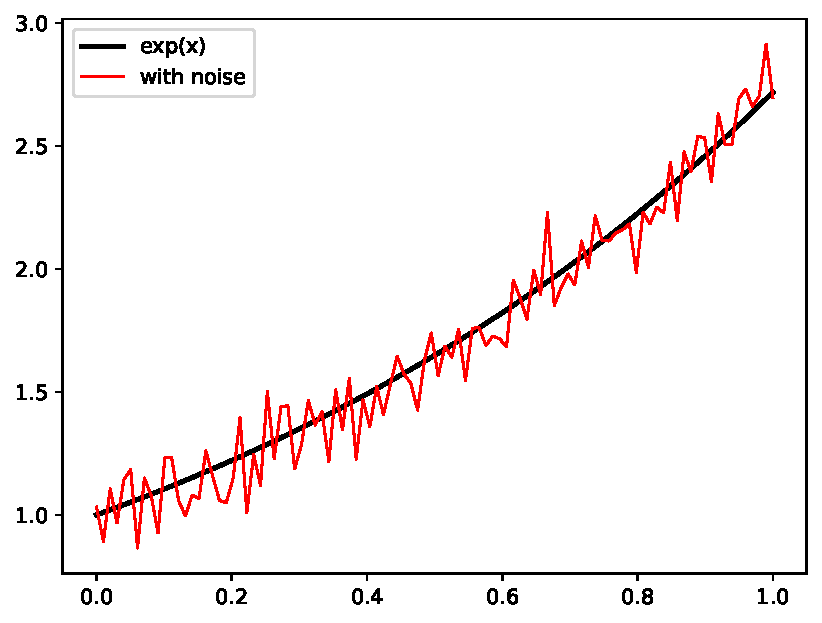
\includegraphics[width=0.5\textwidth]{./figures/exp_with_noise.pdf}
  \caption{An exponential function with random noise.}\label{fig:exp_with_noise}
\end{figure}

\end{document}
